\chapter{Test Plan}
\section{Test Strategy}

The tests carried out in this project are divided into two main categories. For the project an Incremental Testing approach is used. In incremental testing a combination of bottom-up and top-down Testing is conducted. At the end of each Sprint there should be a Potentially Shippable Product Increment based on the Sprint goal. To verify a User Story, the specific Acceptance Criterion has to be determined. These are formulated based on the Agile GIVEN, WHEN and THEN-method, also called Gherkin Syntax. This method makes it easy to test small parts of the system. There will be performed a set of verification tests for the most important User Stories, the tests are passed if the Acceptance Criteria is met. Verification tests helps to determine if the product is built right in accordance to the backlog.\\
\\
For research testing, statistical hypothesis tests are conducted. A hypothesis test is a statistical test that is used to determine whether there is enough evidence in a sample of data to infer that a certain condition is true for the entire population \cite{statistikk3}. For this project the main goal is to gain information about the characteristics of a quadcopter with variable pitch propellers. This is done by comparing the attributes of variable pitch against fixed pitch propellers on a quadcopter. \\

\newpage

\subsection{Gherkin Syntax}
Gherkin Syntax is used to formulate Acceptance Criteria for User Stories. The benefit of this approach is that the criterion is written as a readable story that describes a wanted behavior, which makes testing easier \cite{ref7}. Gherkin Syntax is often used in software development and testing, but for this project it gives an understandable description of a wanted behaviour for all parts of the system. In Tab. \ref{tab:gherkin} the syntax adopted is explained. 
\begin {table}[h]
    \begin{center}
    \caption {Gherkin Syntax} 
    \label{tab:gherkin} 
    \begin{tabular}{|l|l|}\hline 
\rowcolor{white} GIVEN   &   Some Precondition \\ \rowcolor{gainsboro}
    AND     &   Some Other Precondition        \\
    WHEN    &   Some Action        \\ \rowcolor{gainsboro}
    AND     &   Yet Another Action        \\
    THEN    &   Some Testable Outcome is Achieved       \\ \rowcolor{gainsboro}
    AND    &   Something else we can Test Happens too.   \\
    \hline
    \end{tabular}
    \end{center}
\end{table}
\\
From this syntax a Test Case with a testable Acceptance Criterion is created. An Acceptance Criterion relates back to the User Story, the User Story relates back to a Product Backlog Item, and the Product Backlog Item relates back to a customer need. In Fig. \ref{fig:ACmatrix} the Acceptance Criteria Matrix for this project is displayed. \\\\(See TraceabilityMatrix\_Ver4.0.xlsx on USB for full version).

\begin{figure}[h]
    \centering
        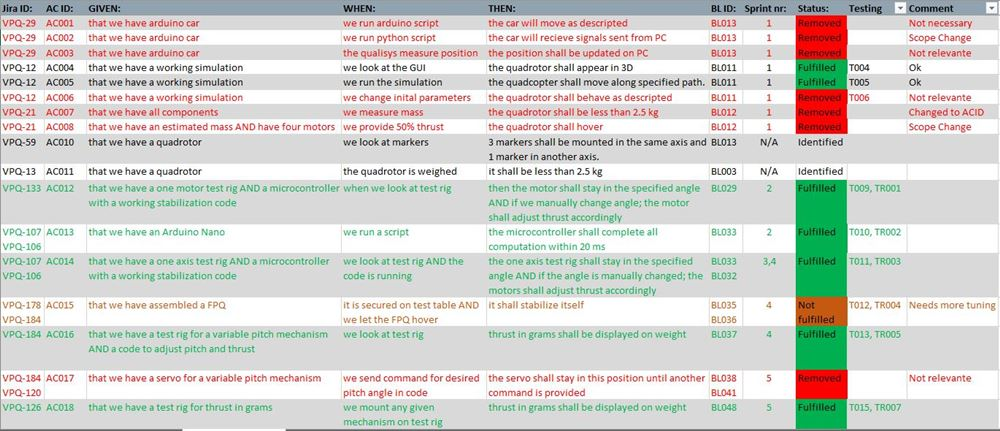
\includegraphics[width=1\textwidth]{VAPIQ-PICTURES/ACmatrix}
        \caption{Acceptance Criteria Tractability Matrix}
        \label{fig:ACmatrix}
\end{figure}


\newpage

\section{Test Case Setup}
The template presented below functions as a Verification record where the Acceptance Criterion is tested. This represents the Test Case where each card states a unique test ID. The Test Case displays which Acceptance Criteria, Backlog Item and JIRA ID it relates to, and in which Sprint the Acceptance Criteria has been fulfilled. It also displays which verification procedures are used and the results of the tests. The Test Cases have been given an ID in the form of TXXX, where the XXX will be numbers. Each Test Case will be enumerated chronologically as the project progresses. \\
\\
\testcard{TXXX}{ACXXX}{X}{BLXXX}{VPQ-XX}
         {\shortstack[l]{GIVEN, WHEN, THEN}}
         {\shortstack[l]{}}
         {\shortstack[l]{TRXXX}}
         {\shortstack[l]{}}

\subsection*{Verification Procedure}
In the Verification Procedure row shown above the test method is stated and a procedure for testing is generated. Sometimes a Static Testing approach will be implemented and other times a Dynamic approach. 
\\
\subsection*{Results and Reports}
In the Result(s)/Reports(s) row the outcome of the test is stated. Some tests are more extensive and demands a more detailed procedure. In these situations a Test Report is generated. The Test Report will be referred to in the Result(s)/Report(s) row as shown in the template above. The Test Report has been given an ID in the form of TRXXX, where the XXX will be numbers. Each Test Report is enumerated chronologically as the project progresses. \\ 
\\
\begin{comment}
The test results are crucial to be able to verify our system and research. The test results gives us feedback if something is or is not functioning as the Acceptance Criteria specifies. Continuous testing of every criterion will help the verification of the system. \\
\end{comment}

\newpage

\subsection*{Test Traceability Matrix}
In Fig. \ref{fig:Tmatrix} the Test Traceability Matrix for this project is displayed.\\\\ (See TraceabilityMatrix\_Ver3.0.xlsx on USB for full version).

\begin{figure}[h]
    \centering
        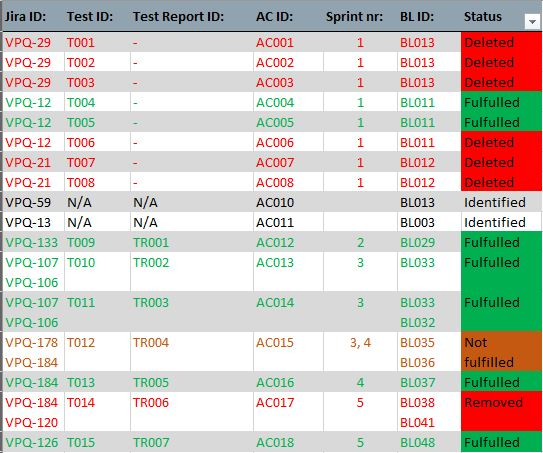
\includegraphics[width=0.7\textwidth]{VAPIQ-PICTURES/Tmatrix}
        \caption{Test Taceability Matrix}
        \label{fig:Tmatrix}
\end{figure}

\newpage

\subsection*{Test Processes}
In Fig. \ref{fig:testsetup} a simple illustration of how the Verification Test process works for one Product Backlog Item is displayed. The Test Cases and Test Reports will include all the information needed for verification of the User Story.\\
\\
\begin{figure}[h]
    \centering
        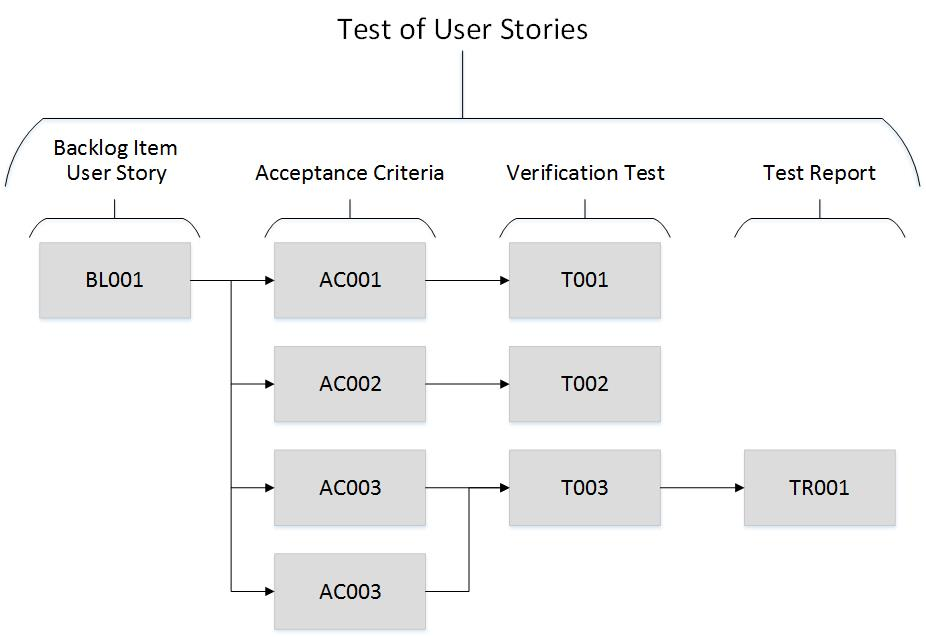
\includegraphics[width=0.8\textwidth]{VAPIQ-PICTURES/testdocbild}
        \caption{Test of Backlog Item}
        \label{fig:testsetup}
\end{figure}
\\
Fig. \ref{fig:testsetup} shows an example of how to test User Stories. This figure does not related to any performed tests.\\

\newpage
In Fig. \ref{fig:testsetup2} a simple illustration of how the Verification Test Process works for one Sprint Backlog. 

\begin{figure}[h]
    \centering
        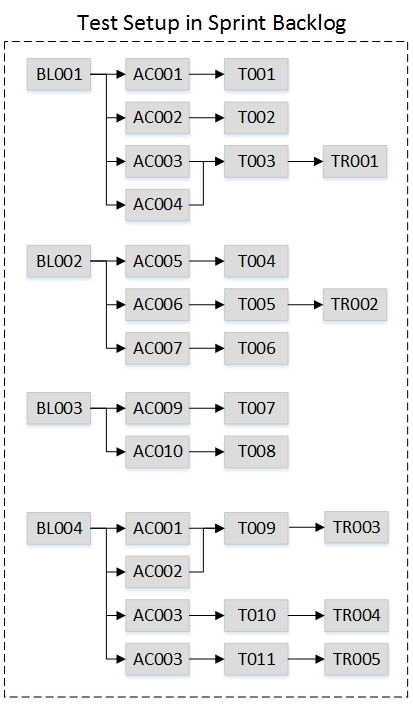
\includegraphics[width=0.55\textwidth]{VAPIQ-PICTURES/testdocbild2}
        \caption{Test Process for Sprint Backlog}
        \label{fig:testsetup2}
\end{figure}
\noindent
Fig. \ref{fig:testsetup2} shows an example of how tests are conducted in one Sprint Backlog. This figure is not related to any performed tests.\\
\newpage